% Build from reports/: TEXINPUTS=../docs: xelatex -jobname=Report main.tex
\documentclass[conference,a4paper]{IEEEtran}
\usepackage{fontspec}
\setmainfont{Times New Roman}[SmallCapsFont=TeX Gyre Termes]
\setsansfont{Arial}
\setmonofont{Noto Sans Mono}
\usepackage[vietnamese]{babel}
\usepackage{amsmath,amssymb,booktabs,array,graphicx,algorithmic,url}
\usepackage[hidelinks,unicode]{hyperref}
\graphicspath{{figures/fashion/}{../docs/report_tv2/figures/}}
\renewcommand{\figurename}{Hình}
\renewcommand{\tablename}{Bảng}
\renewcommand{\refname}{Tài liệu tham khảo}
\renewcommand{\algorithmicrequire}{\textbf{Đầu vào:}}
\renewcommand{\algorithmicensure}{\textbf{Đầu ra:}}
\newcommand{\bv}{\texttt{BitVector}}
\newcommand{\st}{\texttt{Set}}
\newcommand{\pending}{\textemdash}
\makeatletter
\newenvironment{reportfigure}{\par\medskip\noindent\begin{minipage}{\columnwidth}\def\@captype{figure}\centering}{\end{minipage}\par\medskip}
\newenvironment{reporttable}{\par\medskip\noindent\begin{minipage}{\columnwidth}\def\@captype{table}\centering}{\end{minipage}\par\medskip}
\makeatother
\newcommand{\pendingplot}[2]{\fbox{\begin{minipage}[c][#1][c]{0.94\columnwidth}\centering\small #2\par\medskip\textit{Khung dành cho biểu đồ sau khi chốt số liệu.}\end{minipage}}}
\begin{document}
\selectlanguage{vietnamese}
\renewcommand{\refname}{Tài liệu tham khảo}
\pagestyle{plain}
\title{Cài đặt và tối ưu Eclat bằng Julia\\cho phân tích giỏ hàng và khai thác mẫu trực quan}
\author{\IEEEauthorblockN{Trung \qquad Khang \qquad Duy}
\IEEEauthorblockA{Đồ án môn Khai phá dữ liệu\\Trường Đại học Khoa học Tự nhiên, ĐHQG-HCM}}
\maketitle
\begin{abstract}
Khai thác tập mục phổ biến tìm các tổ hợp thường cùng xuất hiện trong cơ sở
dữ liệu giao dịch. Báo cáo trình bày cài đặt Eclat bằng Julia với hai biểu
diễn tập định danh giao dịch: Set và BitVector. Thuật toán được xây dựng
theo mô tả của Zaki, sử dụng giao TID-set và duyệt theo chiều sâu; phiên
bản tối ưu lọc singleton trước khi cấp phát vector bit. Bộ kiểm thử đối
chiếu từng itemset và support count với SPMF trên năm cơ sở dữ liệu, đồng
thời dùng phép đếm vét cạn độc lập trên dữ liệu nhỏ. Thực nghiệm được thiết
kế trên Chess, Mushroom, Retail và T10I4D100K để đánh giá thời gian thực thi
(runtime), đỉnh bộ nhớ thường trú (Peak RSS),
khả năng mở rộng và ảnh hưởng của độ dài giao dịch. Hai ứng dụng dùng cùng
core: Groceries sinh luật kết hợp và xếp top 10 theo lift; Fashion-MNIST
biểu diễn ảnh bằng túi từ thị giác rồi khai thác các tổ hợp từ thị giác
(visual words).
Bản thảo đã có kết quả Groceries và correctness; các số đo hiệu năng cùng
kết quả lần chạy Fashion-MNIST 70.000 ảnh đang để trống chờ xác nhận.
\end{abstract}
\begin{IEEEkeywords}
Eclat, frequent itemset mining, Julia, BitVector, luật kết hợp, visual words.
\end{IEEEkeywords}
\noindent\textit{Quy ước bản thảo.} Dấu \pending{} trong bảng kết quả nghĩa
là chưa điền số liệu, không phải kết quả bằng 0 hoặc thất bại. Các hình có
khung ``chờ số liệu'' chỉ chỉ rõ nội dung cần đo. Không dùng số liệu
benchmark cũ hay kết quả demo 1.000 ảnh để thay cho lần đo đang chờ.

\section{Thuật toán Eclat và tối ưu hóa}
\label{sec:tv1}

\subsection{Bài toán và lựa chọn thuật toán}
Cho cơ sở dữ liệu giao dịch $D=(t_1,\ldots,t_N)$ trên tập item $I$ có $M$ phần tử. Mỗi $t_j\subseteq I$ là một giao dịch; hai giao dịch có nội dung giống nhau vẫn được tính riêng. Với tập item $X\subseteq I$, \emph{support count} (số giao dịch chứa $X$) và \emph{relative support} (độ hỗ trợ tương đối) được định nghĩa:
\begin{equation}
 c(X)=|\{j:X\subseteq t_j\}|,\qquad s(X)=\frac{c(X)}{N}.
 \label{eq:tv1-support}
\end{equation}
Với $N>0$ và ngưỡng $s\in(0,1]$, bài toán \emph{frequent itemset mining} (khai thác tập phổ biến) yêu cầu tìm mọi $X\ne\varnothing$ thỏa $c(X)\ge c_{\min}$, trong đó $c_{\min}=\lceil s N\rceil$. Chẳng hạn, $N=5$ và $s=0{,}5$ cho $c_{\min}=3$; dùng phép làm tròn xuống sẽ giữ sai các tập chỉ xuất hiện hai lần.

Cài đặt sử dụng Eclat theo mô tả của Zaki~\cite{zaki}, với \emph{vertical representation} (biểu diễn dọc) và \emph{depth-first search}, DFS (duyệt theo chiều sâu). Apriori~\cite{agrawal} sinh ứng viên theo từng mức, còn Eclat tính support qua giao các tập định danh giao dịch. Cơ chế này cho phép khảo sát hai cấu trúc dữ liệu \texttt{Set} và \texttt{BitVector} trong Julia~\cite{julia} trên cùng quy trình duyệt. SPMF cung cấp cài đặt tham chiếu độc lập để kiểm chứng~\cite{spmf}.

\subsection{Biểu diễn dọc và nguyên tắc mở rộng}
Với mỗi $X$, đặt $T(X)=\{j:X\subseteq t_j\}$ là \emph{transaction-ID set}, TID-set (tập định danh giao dịch chứa $X$). Khi đó:
\begin{equation}
 T(X\cup Y)=T(X)\cap T(Y),\qquad c(X)=|T(X)|.
 \label{eq:tv1-intersection}
\end{equation}
Ví dụ, với $D=(\{1,2,3\},\{1,3\},\{2,3\},\{1,2\})$, ta có $T(\{1\})=\{1,2,4\}$ và $T(\{2\})=\{1,3,4\}$. Vì vậy $T(\{1,2\})=\{1,4\}$, cho support count bằng 2. Nếu $s=0{,}5$, tập $\{1,2\}$ phổ biến nhưng $\{1,2,3\}$ không phổ biến vì chỉ xuất hiện một lần.

Các item được sắp theo ID tăng dần. Tại tiền tố $P$, danh sách mở rộng chứa các cặp $(i,T(P\cup\{i\}))$. Những tập có chung tiền tố tạo thành một \emph{equivalence class} (lớp tương đương); mỗi nhánh chỉ ghép item với các item đứng sau nó. Support có tính \emph{anti-monotonicity} (phản đơn điệu): nếu $X\subseteq Y$ thì $T(Y)\subseteq T(X)$, suy ra $c(Y)\le c(X)$. Do đó, khi một phép giao cho support nhỏ hơn $c_{\min}$, toàn bộ nhánh mở rộng tương ứng được loại.

\subsection{Quy trình khai thác và tính đúng đắn}
Đầu tiên, thuật toán dựng TID-set của từng item, giữ các singleton đạt $c_{\min}$ và sắp theo ID. Sau đó gọi thủ tục trong Bảng~\ref{tab:tv1-pseudocode} với tiền tố rỗng. TID-set của mỗi ứng viên đã bao gồm điều kiện xuất hiện của toàn bộ tiền tố, nên phép giao ở bước 7 tạo đúng TID-set cho tập mở rộng.

\begin{table}[t]
\caption{Giả mã DFS dùng chung cho hai phiên bản Eclat.}
\label{tab:tv1-pseudocode}
\begin{minipage}{\columnwidth}
\small
\begin{algorithmic}[1]
\REQUIRE Tiền tố $P$; danh sách $C=[(i,A_i)]$ tăng theo ID, với $A_i=T(P\cup\{i\})$, $|A_i|\ge c_{\min}$; ngưỡng $c_{\min}$.
\ENSURE Bổ sung mọi tập phổ biến thuộc nhánh $P$ vào $R$.
\FOR{mỗi vị trí $a$ trong $C$}
  \STATE $(i,A)\gets C[a]$; $Q\gets P\cup\{i\}$
  \STATE $R[Q]\gets |A|$
  \STATE $C'\gets [\,]$
  \FOR{mỗi vị trí $b>a$ trong $C$}
    \STATE $(j,B)\gets C[b]$
    \STATE $H\gets A\cap B$
    \IF{$|H|\ge c_{\min}$}
      \STATE Thêm $(j,H)$ vào $C'$
    \ENDIF
  \ENDFOR
  \IF{$C'\ne[\,]$}
    \STATE Gọi EclatDFS$(Q,C',c_{\min},R)$
  \ENDIF
\ENDFOR
\end{algorithmic}
\end{minipage}
\end{table}

\textit{Đúng support.} Ở gốc, mỗi TID-set được dựng trực tiếp từ giao dịch. Nếu các TID-set tại một mức là đúng, công thức~\eqref{eq:tv1-intersection} bảo đảm tập ở mức kế tiếp cũng đúng. Do đó mọi support xuất ra đều bằng số giao dịch thực sự chứa tập item.

\textit{Đầy đủ và không lặp.} Mỗi tập item có duy nhất một thứ tự tăng dần. Nếu tập đó phổ biến, mọi tiền tố của nó cũng phổ biến theo tính phản đơn điệu, nên đường mở rộng tương ứng không bị cắt bỏ. Quy tắc chỉ ghép với item đứng sau bảo đảm đường này được duyệt đúng một lần. Thuật toán vì vậy xuất toàn bộ tập phổ biến, không sinh hoán vị trùng.

\subsection{Phiên bản cơ sở sử dụng Set}
Phiên bản cơ sở trong \texttt{EclatBaseline.jl} lưu TID-set bằng \texttt{Set\{Int\}}. Một lượt quét loại item lặp trong mỗi giao dịch rồi gắn TID vào từng item. DFS dùng \texttt{intersect} để sinh nhánh con. Biểu diễn này chỉ lưu các TID xuất hiện thực tế; chi phí bộ nhớ bao gồm các số nguyên và cấu trúc bảng băm.

\subsection{Các kỹ thuật tối ưu đã cài đặt}
\textit{Biểu diễn TID-set bằng BitVector.} Tệp \texttt{EclatOptimized.jl} biểu diễn TID-set bằng vector $N$ bit: bit thứ $j$ bằng 1 khi giao dịch $j$ chứa item. Phép \texttt{.\&} tạo giao, còn \texttt{count} đếm bit bật. Phép giao xử lý đồng thời nhiều bit trong một từ máy, với hiệu quả phụ thuộc mật độ TID-set và độ dài vector.

\textit{Lọc singleton trước khi cấp phát.} Trước khi cấp vector, chương trình đếm support từng item; biến \texttt{last\_seen\_tid} bảo đảm một giao dịch chỉ đóng góp một lần cho mỗi item. Chỉ các item đạt $c_{\min}$ mới được cấp \texttt{BitVector}; lượt quét thứ hai điền các bit tương ứng. Tất cả ID đều được kiểm tra hợp lệ trong lượt đếm, kể cả item sau đó bị loại.

Nếu có $F_1$ singleton phổ biến, phần vector ban đầu giảm từ $MN$ xuống $F_1N$ bit, chưa tính cấu trúc quản lý. Trên Retail tại $s=4\%$, chỉ 7 trong 16.470 item quan sát được đạt ngưỡng. Lọc trước cấp phát tránh tạo vector cho 16.463 item còn lại. Đổi lại, phương án này cần thêm một lượt đọc giao dịch và hai từ điển đếm/ghi nhận TID gần nhất. Lợi ích cần được xét cùng chi phí tiền xử lý, không chỉ kích thước vector.


Cả hai phiên bản sử dụng tính phản đơn điệu để tỉa ứng viên dưới ngưỡng. Khác biệt thực nghiệm nằm ở biểu diễn TID-set và thời điểm cấp phát vector; tập itemset và support đầu ra được giữ nguyên.

\subsection{Phân tích độ phức tạp}
Gọi $E=\sum_{j=1}^{N}|t_j|$ là tổng số lần xuất hiện item trong dữ liệu đầu vào, $w$ là số bit mỗi từ máy và $F$ là số tập phổ biến. Dựng biểu diễn Set có thời gian kỳ vọng $O(E)$, giả sử thao tác bảng băm có chi phí kỳ vọng hằng số. Phiên bản BitVector cần $O(E+F_1\lceil N/w\rceil)$ cho đếm, cấp vector và điền bit; trạng thái đếm dùng $O(M)$ bộ nhớ. Các cận này chưa gồm sắp xếp ID, có chi phí $O(M\log M)$ ở baseline hoặc $O(F_1\log F_1)$ sau lọc ở phiên bản BitVector.

Một phép giao Set có chi phí kỳ vọng tỷ lệ với kích thước toán hạng nhỏ hơn; giao và đếm BitVector cần $O(\lceil N/w\rceil)$ thao tác trên các từ máy. BitVector có thể tận dụng xử lý theo từ máy khi TID-set dày, trong khi dữ liệu thưa làm tăng tỷ lệ bit 0 phải quét. Sự đánh đổi này được đánh giá thực nghiệm ở Chương II.

Gọi $\mathcal{J}$ là tập các phép giao thực sự được DFS thực hiện, và $K=\sum_{X\text{ phổ biến}}|X|$ là tổng độ dài khóa kết quả. Ngoài tiền xử lý, thời gian gồm tổng chi phí các phép giao trong $\mathcal{J}$, quản lý ứng viên, sao chép tiền tố và lưu kết quả. Riêng phiên bản BitVector, phần giao/đếm có cận $O(|\mathcal{J}|\lceil N/w\rceil)$. Trường hợp xấu nhất $F=2^M-1$, nên không có cận đa thức theo $N,M$ cho việc liệt kê mọi tập phổ biến.

Bộ nhớ TID-set ban đầu của baseline tỷ lệ với số cặp item--TID khác nhau, tối đa $O(E)$; phần vector của bản tối ưu dùng $O(F_1N)$ bit. Bộ nhớ tổng còn gồm dữ liệu đầu vào, các danh sách ứng viên đang sống trên ngăn xếp DFS và kết quả. Độ sâu đệ quy tối đa là $F_1$; lưu từ điển kết quả cần $O(F+K)$ ô lưu trữ. Vì thế, giới hạn bộ nhớ ban đầu không phải giới hạn bộ nhớ cực đại của cả thuật toán.

\subsection{Tích hợp, I/O và dòng lệnh}
Module \texttt{EclatFIM} nhận giao dịch kiểu \texttt{Vector\{Vector\{Int\}\}} với ID nguyên dương. Item lặp chỉ tính một lần; giao dịch trùng vẫn có TID riêng và giao dịch rỗng vẫn góp vào $N$. Kết quả là \texttt{Dict\{Tuple\{Vararg\{Int\}\},Int\}}, khóa tăng dần và giá trị là support count. Julia phân phối theo kiểu đối số: \texttt{mine(T, 0.01; backend=:set)} nhận tỷ lệ, còn \texttt{mine\_count(T, 99; backend=:bitvector)} nhận số đếm. Đặc biệt, \texttt{mine(T, 1)} là count 1, còn \texttt{mine(T, 1.0)} là tỷ lệ 100\%. API số đếm hỗ trợ giới hạn độ dài, deadline và số kết quả; các giới hạn này không phải kỹ thuật tăng tốc được đo trong báo cáo.

\texttt{SPMFIO.jl} đọc một giao dịch mỗi dòng và ghi itemset theo dạng \texttt{1 2 \#SUP: 3}. CLI nhận minsup tương đối, backend và đường dẫn. Ví dụ sau là một lệnh, viết thành nhiều dòng để dễ đọc:
\begin{quote}\small\ttfamily
julia --project=. scripts/eclat\_cli.jl\par
\quad --input INPUT.txt --minsup 0.01\par
\quad --backend bitvector\par
\quad --output OUTPUT.txt
\end{quote}

\subsection{Kiểm thử và đối chiếu SPMF}
Bộ kiểm thử bao phủ support biên, dữ liệu rỗng, giao dịch trùng, item trùng, thứ tự item, ID sai và hai backend. Ngoài ví dụ xác định trước, 40 cơ sở dữ liệu nhỏ sinh với seed 20261116 được kiểm tra ở ba ngưỡng $0{,}2$, $0{,}5$ và $1{,}0$. Đáp án độc lập được tạo bằng vét cạn các tập con và đếm trực tiếp trên giao dịch, giúp tránh trường hợp hai backend cùng mắc một lỗi.

Đối chiếu SPMF kiểm tra toàn bộ từ điển tập item và support, không chỉ tổng số kết quả. Một cấu hình đạt khi không thiếu tập, không thừa tập và không sai support. Bộ test đọc đáp án SPMF đã lưu, không tự sinh đáp án bằng Eclat của nhóm. Các dòng metadata của đáp án được bỏ qua trước khi chuẩn hóa itemset. Năm CSDL đầy đủ gồm Groceries, Chess, Mushroom, Retail và T10I4D100K đều đã ghi nhận khớp 100\% ở cả hai backend; bảng cấu hình và kết quả được trình bày tại Chương II.

Lệnh \texttt{julia --project=. test/runtests.jl} thực hiện kiểm thử toàn package, gồm cả các ứng dụng. Lần chạy ngày 24/11/2026 trên Julia 1.13.3/Linux ghi nhận 569/569 assertions đạt; phép đối chiếu trên năm CSDL khớp 100\% cho cả hai phiên bản. Script \texttt{scripts/prepare\_data.jl} tải dữ liệu và xác minh SHA-256 trước khi chuẩn hóa. Kiểm thử dừng khi thiếu đầu vào để duy trì đầy đủ các trường hợp đối chiếu.

\subsection{Đánh giá tối ưu và giới hạn}
Hiệu quả của hai kỹ thuật được đánh giá ở Chương II theo thời gian toàn tiến trình, Peak RSS và thời gian khai thác sau warm-up. Các kết quả Colab cho thấy mức cải thiện phụ thuộc dữ liệu và phạm vi đo.

So sánh hai phiên bản hoàn chỉnh đánh giá tác động kết hợp của bitset và lọc singleton. Việc định lượng đóng góp từng thành phần đòi hỏi thí nghiệm loại bỏ từng kỹ thuật trong cùng điều kiện. Peak RSS phản ánh tổng bộ nhớ tiến trình, bao gồm môi trường Julia, dữ liệu vào, TID-set và kết quả.

Cài đặt hiện tại cấp phát kết quả giao mới và giữ toàn bộ itemset trong từ điển. Số tập phổ biến lớn vì vậy có thể làm tăng mạnh cả thời gian lẫn bộ nhớ. Tái sử dụng bộ đệm theo mức DFS và chọn biểu diễn theo mật độ là hai hướng mở rộng chưa được triển khai trong phiên bản được đánh giá.

\section{Thực nghiệm và đánh giá}
\label{sec:benchmark}
\subsection{Câu hỏi thực nghiệm và phạm vi}
Thực nghiệm xét ba câu hỏi. Thứ nhất, hai biểu diễn TID-set có xuất đúng
toàn bộ itemset và support so với SPMF hay không? Thứ hai, thay Set bằng
BitVector có giảm runtime và Peak RSS trên các loại dữ liệu khác nhau
hay không? Thứ ba, số giao dịch và độ dài giỏ tác động thế nào đến chi phí
khai thác? Correctness và hiệu năng được kiểm tra riêng: output đúng
không tự bảo đảm phương pháp đo công bằng.

Thiết kế gồm bốn nhóm: runtime và output size theo minsup; Peak RSS ở
minsup giữa dải; scalability theo số giao dịch; và dữ liệu tổng hợp tăng
độ dài giỏ. Mỗi nhóm giữ những biến còn lại cố định trong phạm vi thiết kế.
SPMF Eclat~\cite{spmf} là tham chiếu độc lập, không được gọi bên trong
cài đặt Julia của nhóm.

Các số đo hiệu năng của lần chạy được chọn sẽ điền vào các bảng và khung
hình bên dưới. Bản thảo chưa kết luận backend nào thắng trên dataset nào.
Các lập luận về dense/sparse là cơ chế cần kiểm tra, không phải quan sát
đã có của lần đo đang chờ.

\subsection{Dữ liệu, chuẩn hóa và ngưỡng}
Bốn tập dữ liệu từ FIMI~\cite{fimi} bao phủ giao dịch dày và thưa
(Bảng~\ref{tab:data}). Chess/Mushroom có giỏ dài; Retail có nhiều item
nhưng giỏ ngắn; T10I4D100K là dữ liệu tổng hợp. Số giao dịch lớn không
đồng nghĩa output lớn: phân bố đồng xuất hiện và ngưỡng support còn
quyết định số tổ hợp vượt ngưỡng.

\begin{reporttable}
\caption{Thống kê đầu vào benchmark đã chuẩn hóa; $\bar L$ là độ dài giỏ trung bình.}
\label{tab:data}
\small
\begin{tabular}{lrrr}\toprule
CSDL & $N$ & $M$ & $\bar L$\\\midrule
Chess & 3.196 & 75 & 37,0000\\
Mushroom & 8.124 & 119 & 23,0000\\
Retail & 88.162 & 16.470 & 10,3058\\
T10I4D100K & 100.000 & 870 & 10,1023\\\bottomrule
\end{tabular}
\end{reporttable}

Giữ nguyên giao dịch trùng và thứ tự dòng. Chess/Mushroom giữ ID gốc;
Retail/T10I4D100K cộng 1 vào mọi ID để không còn ID 0. Phép đổi tên một-một
này bảo toàn support; Julia và SPMF phải dùng cùng file sau đổi tên.
Không so output có mapping khác nhau chỉ bằng số lượng itemsets.
Script chuẩn bị dữ liệu kiểm tra SHA-256 của file gốc trước khi chuẩn hóa.

Với tỷ lệ $s$ và $N$ giao dịch, ngưỡng đếm là
\begin{equation}
c_{\min}=\lceil sN\rceil.
\label{eq:threshold}
\end{equation}
Dải ngưỡng trong Bảng~\ref{tab:grids} có bảy điểm mỗi dataset, từ cao
xuống thấp. Ngưỡng tương đối giữ ý nghĩa tần suất giữa các mức kích thước
khác nhau, còn ngưỡng đếm thay đổi theo $N$. Nếu thay dải ngưỡng sau pilot,
cần lưu cấu hình cuối cùng trước khi chạy các lượt chính thức.

\begin{reporttable}
\caption{Dải minsup, đơn vị phần trăm; điểm thứ tư dùng cho Peak RSS.}
\label{tab:grids}
\footnotesize
\begin{tabular}{lp{0.65\columnwidth}}\toprule
CSDL & Bảy ngưỡng từ cao xuống thấp\\\midrule
Chess & 95; 92,5; 90; 87,5; 85; 82,5; 80\\
Mushroom & 95; 90; 80; 70; 60; 50; 40\\
Retail & 10; 8; 6; 4; 2; 1; 0,5\\
T10I4D100K & 3; 2,5; 2; 1,5; 1; 0,75; 0,5\\\bottomrule
\end{tabular}
\end{reporttable}

\subsection{Môi trường và phương pháp đo}
Mọi backend chạy trên cùng máy, cùng đầu vào và một luồng Julia. Khi chốt
số liệu, Bảng~\ref{tab:environment} phải được điền từ metadata của chính
lần đo đó. Không lấy cấu hình máy Windows của kết quả cũ điền cho Colab
hoặc máy Linux khác. Ghi riêng phiên bản Julia, Java và hash JAR SPMF;
tên thuật toán trong log không xác định phiên bản thư viện.

\begin{reporttable}
\caption{Môi trường của lần đo được chọn; \pending{} là chờ cập nhật.}
\label{tab:environment}
\small
\begin{tabular}{lp{0.43\columnwidth}}\toprule
Thuộc tính & Giá trị\\\midrule
Hệ điều hành, kiến trúc & \pending\\
CPU, số CPU logic, RAM & \pending\\
Julia, Java, SHA-256 JAR & \pending\\
Ngày đo, commit nguồn & \pending\\
Luồng Julia & 1\\
Số lượt ghi nhận/cấu hình & 5\\\bottomrule
\end{tabular}
\end{reporttable}

\textit{Runtime toàn tiến trình.} Mỗi mẫu tạo tiến trình mới, gồm khởi
động runtime, JIT, đọc dữ liệu, dựng TID-set, mining và ghi output.
Có một lượt chuẩn bị không ghi nhận cho mỗi chương trình; năm lượt đo
sau vẫn là tiến trình mới và vẫn tính JIT. Đây không phải phép đo miner
đã warm-up trong cùng tiến trình. Chuẩn hóa input và so sánh correctness
thực hiện ngoài đồng hồ.

\textit{Thời gian riêng miner.} Scalability và độ dài giao dịch dùng một
lượt warm-up trên đúng CSDL/cùng minsup trong worker, gọi GC trước đo,
rồi đo một lời gọi mine. GC phát sinh bên trong miner vẫn tính vào thời
gian. Phạm vi đo này khảo sát chi phí khai thác; không dùng để so với
runtime SPMF toàn tiến trình ở thí nghiệm khác.

\textit{Bộ nhớ.} Peak RSS là mức bộ nhớ thường trú cao nhất của worker
đến hết mining, đo trước khi sắp xếp/ghi output. Worker warm-up trên toy,
GC, đọc dữ liệu, GC rồi mine. Bộ đếm mức đỉnh không reset, nên đỉnh vẫn
gồm runtime và warm-up. Trên Windows, đại lượng tương ứng lấy từ peak
working set~\cite{windowsrss}. Allocation tích lũy hay kích thước object
Julia không thay thế cho Peak RSS.

Chạy tuần tự và luân phiên thứ tự giữa các lượt để giảm ảnh hưởng ưu tiên
cố định. Báo cáo trung vị và min--max của năm mẫu, không gọi min--max là
khoảng tin cậy. Nếu máy có workload khác, phải ghi điều kiện đó; không
gộp mẫu của hai môi trường thành một median.

\subsection{Correctness và kiểm thử tự động}
Gọi $R$ là output SPMF, $A$ là output Julia, đều được chuẩn hóa thành
ánh xạ tuple item tăng dần sang số đếm. Một cấu hình đạt khi
\begin{equation}
\operatorname{keys}(A)=\operatorname{keys}(R),\quad
\forall X\in R:\ A[X]=R[X].
\end{equation}
Điều kiện này mạnh hơn bằng số lượng: hai output có thể cùng kích thước
nhưng thiếu/thừa itemset hoặc sai support. Tỷ lệ khớp dùng mẫu số là số
itemsets tham chiếu. Nếu tham chiếu rỗng, chỉ xác nhận đạt khi output cũng
rỗng thay vì chia cho 0.

Bảng~\ref{tab:correct} là correctness đã lưu trên năm CSDL đầy đủ. Đây là
đối chiếu với đáp án SPMF có sẵn, không phải số đo hiệu năng đang chờ.
Test không dùng miner của nhóm tạo đáp án cho chính nó.

\begin{reporttable}
\caption{Correctness đã kiểm chứng: cả hai backend khớp toàn bộ itemset/support.}
\label{tab:correct}
\footnotesize
\begin{tabular}{lrrr}\toprule
CSDL & Minsup (\%) & Itemsets SPMF & Khớp\\\midrule
Groceries & 1 & 333 & 100\%\\
Chess & 87,5 & 1.386 & 100\%\\
Mushroom & 70 & 31 & 100\%\\
Retail & 4 & 18 & 100\%\\
T10I4D100K & 1,5 & 237 & 100\%\\\bottomrule
\end{tabular}
\end{reporttable}

Ngoài reference SPMF, test dùng phép vét cạn tập con trên dữ liệu nhỏ và
kiểm tra input không bị sửa tại chỗ. Những ca rỗng, item trùng, giao dịch
trùng, ngưỡng biên và ID sai giúp tách lỗi parser khỏi lỗi DFS. Log package
569/569 assertions trong README bao gồm cả ứng dụng; đây không phải số
dataset hoặc số lượt SPMF. Trước khi cập nhật hiệu năng, cần chạy lại
correctness trên đúng commit và mapping đầu vào.

\subsection{Runtime và output size theo minsup}
Với mỗi dataset và mỗi ngưỡng ở Bảng~\ref{tab:grids}, chạy Set, BitVector
và SPMF năm lần: tổng số mẫu dự kiến là $4\times7\times3\times5=420$.
Mỗi mẫu phải có runtime, số itemsets và trạng thái đối chiếu đầy đủ.
Bảng~\ref{tab:runtime-pending} là khung tổng hợp tại ngưỡng thấp nhất;
CSV vẫn phải lưu cả 28 cấu hình.

\begin{reporttable}
\caption{Runtime toàn tiến trình tại ngưỡng thấp nhất (s); các ô chờ kết quả.}
\label{tab:runtime-pending}
\footnotesize
\begin{tabular}{lrrrrr}\toprule
CSDL & $s$ (\%) & Set & BV & SPMF & Itemsets\\\midrule
Chess & 80 & \pending & \pending & \pending & \pending\\
Mushroom & 40 & \pending & \pending & \pending & \pending\\
Retail & 0,5 & \pending & \pending & \pending & \pending\\
T10I4D100K & 0,5 & \pending & \pending & \pending & \pending\\\bottomrule
\end{tabular}
\end{reporttable}

\begin{reportfigure}
\pendingplot{37mm}{Runtime theo minsup cho bốn CSDL\\Ba đường: Set, BitVector, SPMF\\Trung vị năm lượt và vùng min--max}
\caption{Vị trí đồ thị runtime toàn tiến trình. Minsup đi từ cao xuống thấp; runtime dùng giây. Chưa có đường dữ liệu trong bản thảo.}
\label{fig:runtime-pending}
\end{reportfigure}

Hình~\ref{fig:runtime-pending} cần cho thấy ba đường trên cùng hệ trục cho
mỗi dataset. Nếu dùng thang log, phải ghi rõ. Chi phí khởi động/JIT có thể
làm runtime không tăng đều ở từng điểm dù output tăng; đường toàn tiến
trình không tách được tốc độ riêng phần giao TID-set của hai ngôn ngữ.

\begin{reportfigure}
\pendingplot{33mm}{Số itemsets theo minsup\\Bốn CSDL; đối chiếu ba chương trình\\Đánh dấu các run không hoàn tất}
\caption{Vị trí đồ thị output size; chỉ điền số lượng của run hoàn tất và đã đối chiếu support.}
\label{fig:counts-pending}
\end{reportfigure}

Với input cố định, hạ minsup không thể làm mất itemset đã phổ biến. Đường
output size trong Hình~\ref{fig:counts-pending} phải không giảm khi đi từ
ngưỡng cao xuống thấp. Nếu vi phạm, cần kiểm tra input, mapping hoặc run
chưa hoàn tất trước khi giải thích hiệu năng. Phân tích dense/sparse cần
xét phân bố support và độ dài itemset, không chỉ số giao dịch.

\subsection{Peak RSS tại minsup trung bình}
Chọn điểm thứ tư của mỗi dải: Chess 87,5\%, Mushroom 70\%, Retail 4\%,
T10I4D100K 1,5\%. Mỗi backend đo trong năm worker riêng, tổng cộng
$4\times2\times5=40$ mẫu. Output sau đo phải khớp reference và backend
còn lại. Mẫu lỗi giữ trạng thái/log, không điền 0 vào ô RAM để tính median.

\begin{reporttable}
\caption{Peak RSS trung vị (MiB); $\Delta_M$ chờ tính từ hai median.}
\label{tab:ram-pending}
\small
\begin{tabular}{lrrr}\toprule
CSDL & Set & BV & $\Delta_M$ (\%)\\\midrule
Chess & \pending & \pending & \pending\\
Mushroom & \pending & \pending & \pending\\
Retail & \pending & \pending & \pending\\
T10I4D100K & \pending & \pending & \pending\\\bottomrule
\end{tabular}
\end{reporttable}

\begin{reportfigure}
\pendingplot{32mm}{Peak RSS tại ngưỡng giữa dải\\Hai cột Set/BitVector cho mỗi CSDL\\Median và min--max, đơn vị MiB}
\caption{Vị trí đồ thị bộ nhớ; không thay Peak RSS bằng allocation hoặc RAM Java tự báo.}
\label{fig:ram-pending}
\end{reportfigure}

Với $\widetilde M$ là median của năm đỉnh tiến trình, mức giảm RAM là
\begin{equation}
\Delta_M=100\left(1-\frac{\widetilde M_{BV}}{\widetilde M_{Set}}\right).
\end{equation}
Giá trị dương nghĩa là median BitVector thấp hơn. Công thức không biến
phần chênh thành RAM riêng thuật toán. Không lấy hiệu Peak RSS trước và
sau mining để suy bộ nhớ miner, vì cả hai đều là high-water mark.

Khi phân tích Bảng~\ref{tab:ram-pending} và Hình~\ref{fig:ram-pending},
cần xét số singleton còn lại. Cấp $N$ bit cho item hiếm có thể lãng phí;
lọc sớm giảm số vector nhưng thêm một lượt quét. Muốn tách riêng tác động
của bitset và lọc singleton cần ablation cùng input và cùng miner.

\subsection{Scalability theo số giao dịch}
Retail có 88.162 giao dịch và nhiều item. Dùng
\texttt{MersenneTwister(20261116)} tạo một hoán vị TID, lấy tiền tố
10\%, 25\%, 50\%, 75\%, 100\%, rồi sắp chỉ số theo thứ tự dòng gốc.
Các tập con lồng nhau; mức 100\% khớp file chuẩn hóa ban đầu.
Không nhân bản giao dịch để làm dataset lớn hơn.

Giữ minsup 4\%, tính lại $c_{\min}$ cho từng tập con. Hai backend đo riêng
mine sau warm-up; mỗi mức lặp năm lần, tổng 50 mẫu.
Bảng~\ref{tab:scale-pending} ghi cả kích thước và ngưỡng đếm để không
hiểu nhầm rằng mọi mức dùng cùng min-count.

\begin{reporttable}
\caption{Scalability Retail: thời gian mine sau warm-up (ms), chờ điền.}
\label{tab:scale-pending}
\footnotesize
\begin{tabular}{rrrrr}\toprule
Tỷ lệ (\%) & $N$ & $c_{\min}$ & Set & BV\\\midrule
10 & 8.816 & 353 & \pending & \pending\\
25 & 22.040 & 882 & \pending & \pending\\
50 & 44.081 & 1.764 & \pending & \pending\\
75 & 66.121 & 2.645 & \pending & \pending\\
100 & 88.162 & 3.527 & \pending & \pending\\\bottomrule
\end{tabular}
\end{reporttable}

\begin{reportfigure}
\pendingplot{33mm}{Scalability Retail\\Trục ngang: số giao dịch\\Trục dọc: mine sau warm-up (ms)}
\caption{Vị trí đồ thị scalability với năm mức dữ liệu lồng nhau.}
\label{fig:scale-pending}
\end{reportfigure}

Sau khi có Hình~\ref{fig:scale-pending}, xét tỷ số tăng thời gian so với
tỷ số tăng $N$ và kiểm tra output size ở mỗi mức. Nếu số itemsets đổi,
thời gian tăng có thể do TID-set lớn hơn lẫn nhiều nhánh DFS hơn. Khớp
đường tuyến tính chỉ mô tả miền đã đo, không chứng minh Eclat tuyến tính
với mọi input và minsup.

\subsection{Ảnh hưởng của độ dài giao dịch}
Sinh $N=5.000$ giao dịch trên $M=64$ item, dùng seed 20261116. Mỗi TID có
một hoán vị riêng của $1{:}64$; lấy 4, 8, 12, 16, 20 item đầu để tạo các
mức độ dài. Vì dùng cùng hoán vị cho một TID, giỏ dài chứa giỏ ngắn tương
ứng. Giữ minsup 5\%, nên $c_{\min}=250$ ở mọi mức.

Không loại giao dịch trùng. Các giỏ trong một CSDL có cùng độ dài $L$,
nên độ dài trung bình bằng $L$ và mật độ bằng $L/M$. Thiết kế tách tác
động của độ dài khỏi $N,M$, nhưng support của nhiều tổ hợp vẫn tăng theo
$L$; đó chính là cơ chế cần khảo sát.

\begin{reporttable}
\caption{Dữ liệu tổng hợp và thời gian mine sau warm-up (ms), chờ điền.}
\label{tab:length-pending}
\footnotesize
\begin{tabular}{rrrrr}\toprule
$L$ & Mật độ (\%) & Itemsets & Set & BV\\\midrule
4 & 6,25 & \pending & \pending & \pending\\
8 & 12,50 & \pending & \pending & \pending\\
12 & 18,75 & \pending & \pending & \pending\\
16 & 25,00 & \pending & \pending & \pending\\
20 & 31,25 & \pending & \pending & \pending\\\bottomrule
\end{tabular}
\end{reporttable}

\begin{reportfigure}
\pendingplot{33mm}{Độ dài giao dịch và chi phí khai thác\\Năm mức $L=4,8,12,16,20$\\Runtime và output size trên hai hệ trục riêng}
\caption{Vị trí đồ thị tác động độ dài; giữ $N$, $M$ và minsup cố định.}
\label{fig:length-pending}
\end{reportfigure}

Với chọn đều $L$ item từ $M$, xác suất một cặp cụ thể có mặt trong giỏ là
\begin{equation}
p_2=\frac{L(L-1)}{M(M-1)}.
\end{equation}
Support kỳ vọng $Np_2$ khoảng 163,7 tại $L=12$ và 297,6 tại $L=16$, nằm
hai phía ngưỡng 250. Đây là tính toán từ thiết kế, chưa phải output quan
sát. Nó giải thích vì sao có thể có bước tăng mạnh số itemsets khi giỏ
dài hơn. Khi điền Hình~\ref{fig:length-pending}, cần kiểm tra dữ liệu có
phù hợp cơ chế này và thời gian bị chi phối bởi giao TID-set hay lưu output.

\subsection{Cách tổng hợp và giới hạn kết luận}
Mỗi cấu hình giữ đủ năm mẫu và trạng thái, sau đó mới tính median. Tỷ số
$t_{Set}/t_{BV}>1$ biểu thị BitVector nhanh hơn trong cùng phạm vi đo; các
thời gian phải dương và cùng đơn vị. Nếu run timeout hoặc OOM, không lấy
thời gian giới hạn như thời gian hoàn tất và không đưa output một phần
vào đối chiếu đầy đủ. Số run thành công trên tổng số dự kiến cần được
trình bày cùng kết quả.

Khi cập nhật, thay đồng thời bảng, hình, môi trường, số lần lặp và nhận
xét. Correctness đúng không chứng minh thiết kế đo công bằng; đo nhanh
nhưng output thiếu cũng không phải cải thiện hợp lệ.

Hai hướng tiếp theo là chọn biểu diễn TID theo mật độ và giảm cấp phát
trong DFS. Hướng thứ nhất dùng cấu trúc thưa cho nhánh ít TID và bitset
cho nhánh dày, tính cả chi phí chuyển biểu diễn. Hướng thứ hai có thể
đếm giao trước hoặc dùng lại bộ đệm theo độ sâu; không được ghi đè TID-set
còn dùng ở nhánh khác. Cả hai là đề xuất chưa được coi là đã triển khai.

Một máy, năm lượt và một seed cho mỗi thiết kế chưa đại diện mọi môi
trường. Kết luận chỉ áp dụng cho dải minsup, dataset và phương pháp đã
ghi; không suy từ đường gần tuyến tính rằng thuật toán có cận đa thức
khi phải xuất mọi tập phổ biến.

\section{Ứng dụng thực tế}\label{sec:applications}
\subsection{Groceries: phân tích giỏ hàng}\label{sec:groceries}
\subsubsection{Bài toán và chuyển đổi dữ liệu}
Ứng dụng phân tích giỏ hàng (market basket analysis) dùng các sản phẩm
thường được mua cùng nhau để sinh luật kết hợp \cite{agrawal}.
Groceries CSV \cite{groceries} có 9.835 giỏ và 169 tên sản phẩm.
Mỗi dòng được đọc như một danh sách có độ dài thay đổi: bỏ khoảng trắng
và item lặp trong giỏ, giữ các giỏ trùng nhau. Vocabulary được sắp theo tên
rồi gán ID dương; mapping ngược dùng để diễn giải kết quả.
Các vector ID sau mã hóa được khai thác bằng Eclat của nhóm.

\subsubsection{Sinh luật và lựa chọn ngưỡng}
Từ mỗi frequent itemset $Z$ có ít nhất hai item, liệt kê các tập con thực
sự, khác rỗng X làm vế trái; vế phải $Y=Z\setminus X$.
Với $c(A)$ là số giỏ chứa toàn bộ A và $N=9.835$, các chỉ số là
\begin{align}
\operatorname{supp}(X\Rightarrow Y)&=\frac{c(X\cup Y)}{N},\\
\operatorname{conf}(X\Rightarrow Y)&=\frac{c(X\cup Y)}{c(X)},\\
\operatorname{lift}(X\Rightarrow Y)&=\frac{\operatorname{conf}(X\Rightarrow Y)}{c(Y)/N}.
\end{align}
Support cho biết độ phổ biến của tổ hợp; confidence cho biết tỷ lệ có Y
trong nhóm giỏ có X; lift so tỷ lệ này với tần suất chung của Y.

Bảng~\ref{tab:params} khảo sát bốn minsup và ba minconf. Minconf được lọc
sau mining nên không làm đổi số itemsets. Khi minsup tăng từ 0,5\% lên 3\%,
số itemsets giảm từ 1.001 xuống 63; tại minconf 50\%, số luật giảm từ 120
xuống 0. Chọn minsup 1\%, minconf 50\% cho cấu hình chính: có 333 itemsets
và 15 luật, đủ để trình bày top 10 nhưng vẫn dễ diễn giải. Hợp hai vế
phải xuất hiện trong ít nhất 99 giỏ theo (\ref{eq:threshold}).

\begin{reporttable}
\caption{Số itemsets và số luật theo minsup, minconf. Ba cột cuối là số luật tại từng minconf.}\label{tab:params}
\centering\footnotesize
\begin{tabular}{rrrrr}\toprule
$s$ (\%) & Itemsets & 30\% & 50\% & 70\% \\\midrule
0,5 & 1001 & 487 & 120 & 1 \\
1,0 & 333 & 125 & 15 & 0 \\
2,0 & 122 & 37 & 1 & 0 \\
3,0 & 63 & 14 & 0 & 0 \\
\bottomrule\end{tabular}
\end{reporttable}

Các luật được xếp giảm dần theo lift, sau đó theo confidence và support
để phân biệt các trường hợp bằng nhau. Việc chọn ngưỡng dựa trên số luật
và khả năng diễn giải trong dữ liệu hiện có, chưa tối ưu theo doanh thu.

\subsubsection{Top 10 luật và ý nghĩa kinh doanh}
Bảng~\ref{tab:rules} giữ nguyên tên sản phẩm của dataset, kèm số đếm và
ba chỉ số. Các luật 1--4 hướng tới \textit{other vegetables}, còn các luật
5--10 hướng tới \textit{whole milk}. Đây là hai nhóm sản phẩm có thể thử
gợi ý theo ngữ cảnh giỏ hàng. Support của các luật chỉ khoảng 1,01--1,45\%,
nên lift cao không đồng nghĩa bao phủ phần lớn các giỏ.

\begin{table*}[!t]
\caption{Top 10 luật Groceries tại minsup 1\%, minconf 50\%, xếp theo lift. Số đếm là số giỏ chứa hợp hai vế; support và confidence theo phần trăm.}\label{tab:rules}
\centering\footnotesize
\begin{tabular}{rp{.31\textwidth}p{.15\textwidth}rrrr}\toprule
\# & Vế trái $X$ & Vế phải $Y$ & Số giỏ & Support & Confidence & Lift \\\midrule
1 & citrus fruit + root vegetables & other vegetables & 102 & 1,037 & 58,62 & 3,030 \\
2 & root vegetables + tropical fruit & other vegetables & 121 & 1,230 & 58,45 & 3,021 \\
3 & rolls/buns + root vegetables & other vegetables & 120 & 1,220 & 50,21 & 2,595 \\
4 & root vegetables + yogurt & other vegetables & 127 & 1,291 & 50,00 & 2,584 \\
5 & curd + yogurt & whole milk & 99 & 1,007 & 58,24 & 2,279 \\
6 & butter + other vegetables & whole milk & 113 & 1,149 & 57,36 & 2,245 \\
7 & root vegetables + tropical fruit & whole milk & 118 & 1,200 & 57,00 & 2,231 \\
8 & root vegetables + yogurt & whole milk & 143 & 1,454 & 56,30 & 2,203 \\
9 & domestic eggs + other vegetables & whole milk & 121 & 1,230 & 55,25 & 2,162 \\
10 & whipped/sour cream + yogurt & whole milk & 107 & 1,088 & 52,45 & 2,053 \\
\bottomrule\end{tabular}
\end{table*}

Xét luật số 1: citrus fruit + root vegetables $\Rightarrow$ other vegetables.
Có 174 giỏ chứa vế trái, trong đó 102 giỏ chứa cả hai vế. Vì vậy support
là $102/9.835\approx1,037\%$, confidence là $102/174\approx58,62\%$.
Other vegetables xuất hiện trong 1.903 giỏ, tương đương 19,35\% toàn bộ
dữ liệu; lift của luật xấp xỉ 3,03. Nghĩa là tỷ lệ có rau khác trong nhóm
giỏ đã có trái cây có múi và rau củ cao khoảng 3,03 lần tỷ lệ chung.

Có thể thử gợi ý rau khác cho các giỏ thỏa điều kiện ở luật 1--4, hoặc
sữa nguyên kem cho các giỏ có tổ hợp sữa chua, rau, bơ, trứng ở luật 5--10.
Khi chọn luật áp dụng, cần xét cả độ phủ: luật 8 dựa trên 143 giỏ, trong
khi luật 5 có 99 giỏ, sát ngưỡng support. Các luật chồng lặp sản phẩm nên
không cộng số giỏ của chúng để ước lượng lợi ích tổng.

\subsubsection{Giới hạn áp dụng}
Luật mô tả đồng xuất hiện trong giỏ hoàn tất, không cho biết thứ tự mua
hoặc quan hệ nhân quả. Dữ liệu không có mã khách, thời gian, giá và khuyến
mãi; top 10 cũng được chọn và mô tả trên cùng CSDL. Vì vậy chưa thể kết
luận gợi ý sản phẩm sẽ làm tăng doanh thu hoặc các luật sẽ ổn định theo thời gian.
Trước khi vận hành, cần đánh giá trên dữ liệu mới và thí nghiệm A/B để đo
chuyển đổi hoặc lợi nhuận. Số đếm và support phải được đọc cùng lift để
tránh đánh giá quá cao các luật ít gặp.

\subsection{Fashion-MNIST: khai thác mẫu trực quan}
\label{sec:fashion}
\subsubsection{Bài toán và phạm vi ứng dụng}
Eclat nhận tập item rời rạc, còn ảnh là một lưới pixel có cấu trúc không
gian. Quyết định chính là chuyển ảnh thành giao dịch mà vẫn truy vết
được item về ảnh gốc. Nhóm dùng túi từ thị giác
(\textit{Bag of Visual Words}, BoVW)~\cite{Sivic03}: mỗi vùng ảnh nhỏ được
gán một visual word, rồi tập mã xuất hiện trong ảnh trở thành giao dịch.
Frequent itemset mô tả tổ hợp visual words thường cùng xuất hiện.

Fashion-MNIST~\cite{Xiao2017} gồm 60.000 ảnh train và 10.000 ảnh test,
mỗi ảnh xám $28\times28$ pixel, chia đều cho mười lớp. Mỗi lớp có 6.000
ảnh train và 1.000 ảnh test. Các lớp gồm T-shirt/top, Trouser, Pullover,
Dress, Coat, Sandal, Shirt, Sneaker, Bag và Ankle boot. Nhãn được giữ
riêng để mô tả kết quả sau mining, không đưa vào descriptor hay tập item.

Bài toán hiện tại là phân tích mô tả, không phải huấn luyện bộ phân loại.
Profile release cố định B0/K32/seed123/S0 và dùng toàn bộ 70.000 ảnh để
học từ điển. Đây là baseline được chọn cho luồng release; chưa có cơ sở
gọi nó là cấu hình tối ưu qua EDA2. Lưới K/seed và spatial encoding là
thí nghiệm riêng, không nhập vào kết quả của profile cố định này.

\subsubsection{Kiểm định dataset và định danh ảnh}
Pipeline tải hoặc dùng lại bốn archive ảnh/nhãn chính thức, đối chiếu
SHA-256, giải nén gzip và đọc IDX. Kiểm tra magic number, số ảnh/nhãn,
kích thước 28$\times$28 và nhãn trong $0{:}9$ giúp phát hiện archive hỏng
hoặc sai bộ dữ liệu. Không chỉ dựa vào tên file hoặc việc giải nén thành
công để xác nhận đúng dữ liệu.

Một ảnh có ID ổn định dạng \texttt{train:<index>} hoặc
\texttt{test:<index>}, với index nguồn bắt đầu từ 0. TID của database bắt
đầu từ 1 và là thứ tự giao dịch, không phải nhãn lớp hoặc mã ảnh. Phân
biệt này tránh nhầm chỉ số mảng Julia bắt đầu từ 1 với vị trí nguồn IDX.
Hai ảnh khác nhau có giao dịch giống nhau vẫn giữ hai TID riêng.

Notebook đầu ghi dataset manifest gồm run ID, số ảnh, shape và hash
archive. Các bước sau chỉ đọc artifacts cùng run và dừng nếu schema, run
identity hoặc hash không khớp. TID/image ID không được dùng như item:
đưa chúng vào tập item sẽ mã hóa danh tính quan sát thay vì nội dung ảnh.

\subsubsection{TC1--TC3: vùng ảnh, lọc nền và descriptor}
Hình~\ref{fig:fashion-pipeline} tóm tắt luồng xây dựng giao dịch. Mỗi ảnh
được chia theo lưới không chồng lấn: patch $4\times4$, stride 4, không
padding. Số vùng trước lọc là
\begin{equation}
\left(\frac{28}{4}\right)^2=49.
\end{equation}
Thứ tự patch là row-major trên lưới $7\times7$; tọa độ hàng/cột và patch ID
được giữ để đối chiếu khi dựng gallery.

\begin{figure*}[t]
\centering
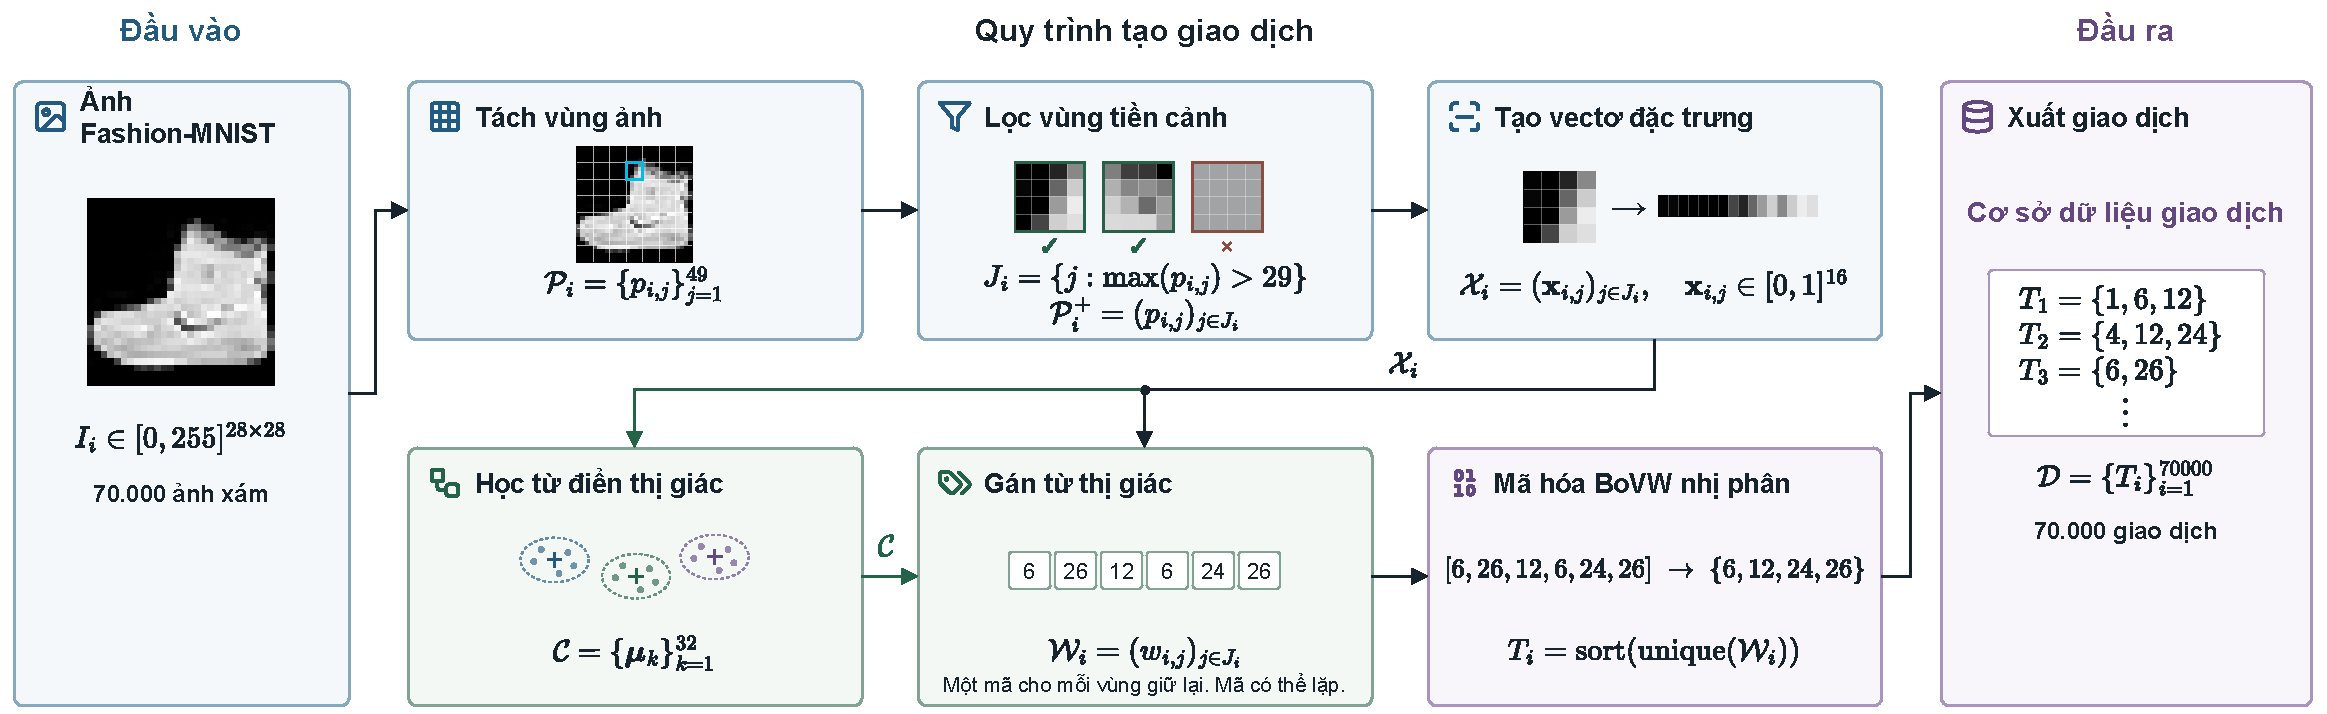
\includegraphics[width=0.98\textwidth]{TC_pipeline.pdf}
\caption{Quy trình dựng giao dịch từ ảnh. Các mã và giao dịch trong sơ đồ chỉ minh họa cấu trúc; TC4 release học một codebook chung từ toàn bộ 70.000 ảnh.}
\label{fig:fashion-pipeline}
\end{figure*}

Một patch $p$ được giữ khi
\begin{equation}
\max_{u,v}p_{u,v}>29.
\label{eq:foreground}
\end{equation}
Đây là điều kiện có ít nhất một pixel lớn hơn 29, không phải mean pixel
lớn hơn 29. Ngưỡng cố định và phép so sánh nghiêm ngặt phải giữ nguyên
giữa các run. Bộ lọc giảm vùng nền gần như đen; nó không bảo đảm mọi
patch còn lại có nghĩa như cổ áo hoặc đế giày.

Với patch giữ lại, descriptor $x_p\in[0,1]^{16}$ là
\begin{equation}
x_p=\frac{\operatorname{vec}(p)}{255},
\end{equation}
trong đó vec đọc 16 pixel theo thứ tự cột và lưu Float32. Thứ tự duyệt
patch trên ảnh và thứ tự flatten bên trong patch là hai quy ước khác
nhau. Dùng cùng quy ước khi reshape centroid về $4\times4$ để tránh đổi
vị trí pixel trong hình diễn giải.

Giả sử ảnh $i$ còn $q_i$ patch sau lọc, tổng descriptor là
$P=\sum_iq_i$, với $0\leq q_i\leq49$. Ma trận có shape $16\times P$.
Cần đối chiếu số cột với số hàng patch metadata, kiểm tra giá trị hữu hạn
và miền $[0,1]$. Không nối nhãn và tọa độ vào vector, vì chúng sẽ đổi
khoảng cách và ý nghĩa visual word đã chốt.

\subsubsection{TC4: học codebook bằng K-means}
B0 dùng K-means full-batch trên toàn bộ descriptors giữ lại, không lấy
mẫu ảnh hoặc descriptor trong profile release. Với $K=32$ centroid
$\mu_1,\ldots,\mu_K$, mục tiêu là giảm
\begin{equation}
J=\sum_{p=1}^{P}\min_{1\leq k\leq K}\|x_p-\mu_k\|_2^2.
\label{eq:kmeans}
\end{equation}
Vòng lặp gán cụm/cập nhật tâm theo K-means~\cite{lloyd} do
Clustering.jl thực hiện~\cite{clustering}; core FIM vẫn là Eclat tự cài
đặt. Khởi tạo dùng K-means++~\cite{kmpp} với seed 123.

\begin{reporttable}
\caption{Cấu hình codebook Fashion release; đây là tham số, không phải kết quả benchmark.}
\label{tab:fashion-config}
\small
\begin{tabular}{lp{0.52\columnwidth}}\toprule
Thuộc tính & Giá trị\\\midrule
Ảnh tham gia fit & Đủ 70.000 ảnh\\
Descriptor & Raw pixels, 16D Float32/255\\
Codebook & B0, full-batch K-means\\
Số cụm và seed & K=32, seed=123\\
Khởi tạo & K-means++\\
Giới hạn vòng lặp & 300\\
Tolerance & $10^{-4}$\\
Khoảng cách & Squared Euclidean\\\bottomrule
\end{tabular}
\end{reporttable}

Bảng~\ref{tab:fashion-config} xác định thí nghiệm phải tái lập. Seed cố
định ngẫu nhiên trong cùng môi trường, nhưng không thay việc ghi phiên
bản thư viện, kiểu số và artifact hash. Kiểm tra centroid shape
$16\times32$, giá trị hữu hạn, occupancy và trạng thái hội tụ. Chạm giới
hạn vòng lặp không được diễn giải như đã hội tụ.

K-means gộp các vùng có khoảng cách pixel nhỏ, nên visual word có thể là
kiểu chuyển tiếp sáng tối thay vì một bộ phận quần áo. Hai ảnh khác lớp
có thể dùng cùng từ; một vật thể cùng lớp có thể đổi mã khi thay độ sáng
hoặc vị trí biên. Đặt tên ngữ nghĩa cho word cần dựa trên patch thật,
không chỉ centroid.

\subsubsection{TC5--TC6: gán từ và mã hóa giao dịch}
Mỗi descriptor nhận mã tâm gần nhất:
\begin{equation}
w_p=\operatorname*{arg\,min}_{1\leq k\leq32}\|x_p-\mu_k\|_2^2.
\end{equation}
Nếu khoảng cách bằng nhau, cài đặt chọn ID nhỏ nhất. Giữ mapping từ mã
về image ID, patch ID và tọa độ. ID cluster không có thứ tự ngữ nghĩa;
word 10 không lớn hơn word 2 theo nghĩa đặc trưng.

Giao dịch S0 của ảnh $I_i$ là
\begin{equation}
T_i=\operatorname{sort}\!\left(\operatorname{unique}
 \{w_p:p\text{ thuộc }I_i\}\right).
\label{eq:s0}
\end{equation}
Mỗi word xuất hiện tối đa một lần trong giỏ. Binary BoVW bỏ qua số patch
lặp và vị trí tương đối. Support đếm số ảnh chứa đủ các word, không đếm
số patch hoặc số lần word xuất hiện.

Nếu không patch nào vượt bộ lọc, ảnh vẫn tạo một giao dịch rỗng. Bỏ ảnh
này sẽ đổi mẫu số support và phân bố lớp. Số giao dịch release phải bằng
70.000, mỗi TID có đúng một image ID. Không áp đặt mọi giao dịch đều
không rỗng nếu chưa đọc kết quả kiểm định.

Bất biến TC6 gồm item thuộc $1{:}32$, item tăng dần và duy nhất, số giao
dịch bằng số ảnh, TID/image ID không lặp. Hai transaction bằng nhau vẫn
là hai quan sát. Codebook và encoding phải cố định trước khi so backend;
fit lại K-means cho mỗi backend sẽ đổi đầu vào của phép so sánh.

\subsubsection{TC7: kiểm định artifact và truy vết}
TC7 đọc lại dữ liệu đã ghi, không chỉ kiểm tra biến trong bộ nhớ.
Bảng~\ref{tab:fashion-artifacts} liệt kê đầu vào của mining/diễn giải.
Manifest ghi run identity, configuration, số ảnh và SHA-256 để phát hiện
ghép nhầm centroid của một lần fit với transaction của lần khác.

\begin{reporttable}
\caption{Artifact truy vết Fashion; các đường dẫn thuộc cùng một run.}
\label{tab:fashion-artifacts}
\footnotesize
\begin{tabular}{lp{0.49\columnwidth}}\toprule
Artifact & Vai trò\\\midrule
Dataset manifest & Nguồn archive, split và hash\\
Transactions JSONL & Một dòng/TID, image ID, tập word\\
Codebook, centroids & Tâm cụm và không gian descriptor\\
Patch assignments & Word gán cho từng vùng ảnh\\
TID/image mapping & Liên kết giao dịch với ảnh nguồn\\
Image metadata & Split, source index và nhãn lớp\\
TC7 manifest & Kiểm định và hash các artifact\\\bottomrule
\end{tabular}
\end{reporttable}

Cùng số hàng chưa đủ xác nhận mapping đúng: thứ tự và ID phải khớp từng
bản ghi. Image ID phải tái tạo được từ split và index nguồn. Với một
hình minh họa, cần tìm được transaction, tọa độ patch và assignment
tương ứng. Gallery đẹp nhưng không nối được bằng chứng chưa xác nhận
được mẫu mined.

\subsubsection{Thiết kế khai thác và đối chiếu}
Hai backend dùng cùng file tại sáu ngưỡng Bảng~\ref{tab:fashion-thresholds}.
Nhãn không tham gia mining. Dùng cùng số luồng, giới hạn tài nguyên và
chính sách ghi output; không cho hai backend cạnh tranh tài nguyên khi đo.

\begin{reporttable}
\caption{Ngưỡng Fashion release trên mẫu số 70.000 ảnh.}
\label{tab:fashion-thresholds}
\small
\begin{tabular}{rr}\toprule
Minsup (\%) & Min-count\\\midrule
80 & 56.000\\60 & 42.000\\40 & 28.000\\
20 & 14.000\\10 & 7.000\\5 & 3.500\\\bottomrule
\end{tabular}
\end{reporttable}

Với itemset $X$, support được audit trực tiếp:
\begin{equation}
c(X)=\sum_{i=1}^{70000}\mathbf{1}[X\subseteq T_i].
\label{eq:fashion-audit}
\end{equation}
So mọi key và count giữa hai backend. Chỉ báo parity đạt khi cả hai run
hoàn tất và toàn bộ ánh xạ giống nhau. Bằng số lượng không thay thế phép
so này; zero kết quả hợp lệ khác với timeout chưa ghi xong file.

\begin{reporttable}
\caption{Kết quả Fashion 70k chờ cập nhật. S/BV là Set/BitVector, RSS tính bằng MiB; các số đo và parity của lần chạy này đều chưa được xác nhận.}
\label{tab:fashion-results}
\footnotesize
\begin{tabular}{rrrrrr}\toprule
$s$ (\%) & Itemsets & $t_S$ (s) & $t_{BV}$ (s) & RSS S/BV & Parity\\\midrule
80 & \pending & \pending & \pending & \pending & \pending\\
60 & \pending & \pending & \pending & \pending & \pending\\
40 & \pending & \pending & \pending & \pending & \pending\\
20 & \pending & \pending & \pending & \pending & \pending\\
10 & \pending & \pending & \pending & \pending & \pending\\
5 & \pending & \pending & \pending & \pending & \pending\\\bottomrule
\end{tabular}
\end{reporttable}

Bảng~\ref{tab:fashion-results} không điền số lịch sử 7.228 như một kết
quả mặc định. Chỉ so với số đó khi transaction hash trùng input của báo
cáo cũ; khác hash ghi không áp dụng. Min-count là tham số đã biết, còn
itemset count, runtime và RSS phải lấy từ artifact hoàn tất.

Đồ thị cần có số itemsets theo minsup, độ dài tối đa và phân bố độ dài,
runtime hai backend và Peak RSS nếu có phép đo hợp lệ. Một lượt mỗi
ngưỡng chỉ mô tả lần chạy đó, chưa chứng minh độ ổn định. Phạm vi đồng
hồ phải ghi rõ trước khi so với Chương II.

\subsubsection{Hai đường thực thi và tình trạng xác minh}
Bộ bốn notebook release nối dataset, transactions, mining và interpretation
bằng manifest. Supervisor dùng Linux user-systemd để giới hạn/theo dõi
worker, ghi trạng thái lỗi tài nguyên và Peak RSS. Run chưa hoàn tất
không được đổi thành parity đạt.

Demo Colab dùng Python kernel gọi Julia và chạy trực tiếp core. Profile
mẫu đã chạy với 1.000 ảnh; profile full gọi cấu hình dựng giao dịch release
70.000 ảnh. Demo đo riêng mine, không có Peak RSS của Fashion. Nó kiểm
tra parity/support, nhưng selection minh họa không thay hợp đồng selector
của Notebook 03--04. Không ghi RSS bằng 0 khi metric chưa đo.

Lần chạy full Colab mới chưa hoàn tất vì runtime bị thu hồi lúc chuẩn bị
môi trường, sau đó dịch vụ từ chối cấp phát tiếp. Điều này chưa xác nhận
lỗi thuật toán, nhưng cũng chưa xác nhận full workflow hoàn tất. Bảng 70k
vì vậy vẫn để trống. Khi cập nhật, ghi rõ đường demo hay bốn notebook
release; không suy từ mẫu nhỏ rằng full-data đã được nghiệm thu.

\subsubsection{Chọn mẫu đại diện}
Selector release gộp và loại trùng itemsets từ các run Set hoàn tất.
Cùng tập xuất hiện ở nhiều ngưỡng phải có support nhất quán; ngưỡng
nguồn là ngưỡng cao nhất đã quan sát. Chia kết quả theo độ dài 1, 2,
$\geq3$ và ba nhóm support thấp/vừa/cao.

Chia nhóm theo thứ hạng các support count phân biệt, để các mẫu cùng số
đếm không bị tách nhóm. Chọn trước từ ba ô (1/cao), (2/vừa), ($\geq3$/thấp)
nếu có ứng viên hợp lệ, rồi điền theo lưới chín ô cố định. Trong mỗi ô
ưu tiên support giảm dần, độ dài, rồi tuple item để không phụ thuộc Dict.

Độ trùng giữa hai mẫu dùng Jaccard:
\begin{equation}
J(X,Y)=\frac{|X\cap Y|}{|X\cup Y|}.
\end{equation}
Chọn tối đa bốn mẫu với ngưỡng 0,80; chưa đủ thì chạy lại một lần ở 0,90.
Bàn giao ba mẫu nếu không có mẫu thứ tư hợp lệ; ít hơn ba phải dừng.
Đây là quy tắc đa dạng hóa mẫu để review, không tối ưu chất lượng phân loại.

Manifest lựa chọn ghi phiên bản quy tắc, thứ tự mẫu, Jaccard, hash catalog
và output nguồn. Không sửa thủ công CSV rồi coi đó là output selector.
Chọn mẫu tự động khác với đánh giá ngữ nghĩa bằng người; trạng thái hai
bước phải được ghi riêng.

\subsubsection{Từ itemset về centroid, patch và ảnh}
Với mỗi word, reshape centroid về $4\times4$ theo thứ tự flatten đã dùng,
đặt cạnh patch thật được gán vào word đó. Giữ tọa độ witness để đánh dấu
vùng trên ảnh gốc. Centroid là trung bình trong không gian descriptor;
nhìn riêng centroid có thể bỏ qua khác biệt giữa các patch cùng cụm.

Với mẫu $X$, lấy toàn bộ ảnh có $X\subseteq T_i$ và kiểm tra số ảnh bằng
support đã audit. Hiển thị tối đa sáu ảnh hỗ trợ theo lựa chọn xác định
và một đối chứng thiếu ít nhất một word nếu có. Không có đối chứng thì
ghi rõ, không tạo ảnh giả.

\begin{reportfigure}
\pendingplot{42mm}{Gallery từ run 70k\\Centroids, patch thật và tọa độ witness\\Ảnh hỗ trợ và ảnh đối chứng}
\caption{Vị trí gallery sau khi có selection manifest và retrieval audit; chưa dùng hình lịch sử như bằng chứng cho run mới.}
\label{fig:fashion-gallery}
\end{reportfigure}

Hình~\ref{fig:fashion-gallery} cần cho thấy mẫu tạo bởi những vùng sáng/tối
nào, gặp ở lớp nào và có nhất quán qua nhiều ảnh không. S0 không giữ vị
trí tương đối, nên không suy ra bố cục lặp lại từ đồng xuất hiện. Nhận
xét về biên cổ áo cần patch/ảnh và reviewer, không thể suy từ word ID.

\begin{reporttable}
\caption{Mẫu 70k chờ lựa chọn/audit; chỉ điền hàng được selector bàn giao.}
\label{tab:fashion-patterns}
\footnotesize
\begin{tabular}{lrrrr}\toprule
Mẫu & Items & Count & Support & Lớp nổi bật\\\midrule
P1 & \pending & \pending & \pending & \pending\\
P2 & \pending & \pending & \pending & \pending\\
P3 & \pending & \pending & \pending & \pending\\
P4 (nếu có) & \pending & \pending & \pending & \pending\\\bottomrule
\end{tabular}
\end{reporttable}

Mỗi hàng Bảng~\ref{tab:fashion-patterns} phải nối tới output Eclat và image
IDs. Người review ghi mức rõ ràng của witness, tính nhất quán hình thái,
nhận xét và hạn chế. Trạng thái bắt đầu là chờ review; pipeline xuất hình
không tự chứng nhận mọi diễn giải đúng.

\subsubsection{Phân bố theo lớp và enrichment}
Sau mining mới nối giao dịch với class label qua stable image ID. Với
$n_c$ ảnh lớp $c$, đặt $c_c(X)$ là số ảnh lớp đó chứa $X$:
\begin{equation}
s_c(X)=\frac{c_c(X)}{n_c},\qquad
E(X,c)=\frac{s_c(X)}{c(X)/N}.
\label{eq:enrichment}
\end{equation}
Mọi ký hiệu dùng cùng run/mẫu số; full dataset có $n_c=7.000$. Kiểm tra
$\sum_c c_c(X)=c(X)$ để phát hiện lỗi mapping. Với support dương,
$E>1$ nghĩa là phổ biến hơn trong lớp so với mức chung, không phải xác
suất phân loại đúng.

Mẫu support cao có thể gặp ở nhiều lớp nên ít phân biệt; mẫu hiếm hơn
có thể tập trung vào một lớp nhưng kém độ phủ. Đọc cùng count, support
theo lớp và enrichment, không chỉ xếp theo $E$. Cùng itemset có thể có
$E\geq2$ cho nhiều lớp; nhiều itemsets có thể chia sẻ phần lớn words.

Bảng lớp/heatmap có thể cho thấy lớp nào chứa nhiều mẫu tập trung, nhưng
đó là phân tích hậu nghiệm. Không dùng nhãn chọn codebook rồi gọi mức
trùng khớp theo lớp là đánh giá độc lập. Nhận xét tổng quát cần ghi cả
quy tắc chọn và số mẫu đã xem.

\subsubsection{Khả năng sử dụng và giới hạn}
Một hướng tiếp theo là biến $m$ frequent itemsets $P_1,\ldots,P_m$ thành
đặc trưng nhị phân của ảnh $I_i$:
\begin{equation}
\phi_j(I_i)=\mathbf{1}[P_j\subseteq T_i],\quad j=1,\ldots,m.
\end{equation}
Các biến mô tả đồng xuất hiện nhiều words, có thể so với BoVW đơn lẻ
bằng cùng một classifier. Hướng đánh giá đề xuất là so BoVW, itemset
features và tổ hợp của chúng với accuracy/Macro-F1. Chưa có kết quả
classifier và không tuyên bố cải thiện.

Codebook release fit cả train và test gốc để mô tả 70.000 ảnh. Dùng
chính dữ liệu đó đánh giá dự đoán có thể gây thiên lệch. Thí nghiệm
classifier độc lập phải fit codebook, mine và chọn features trên train,
cố định phép biến đổi rồi mới áp lên test. Spatial encoding, PCA và
lượng tử hóa là hướng riêng, chưa phải bằng chứng tốt hơn của S0.

Raw descriptor nhạy với thay đổi pixel, không bất biến quay/tỉ lệ.
S0 bỏ vị trí và tần suất patch; bộ lọc nền có thể giữ nhiễu sáng nhỏ.
Giảm minsup tăng chi phí và số mẫu cần review, trong khi nhiều mẫu chỉ
khác một word. Cần nêu các giới hạn này thay vì coi mọi itemset phổ biến
là một bộ phận có nghĩa hoặc quy tắc nhận dạng quần áo.


\subsection{Tổng kết hai ứng dụng}
Hai ứng dụng chia sẻ thuật toán nhưng khác quyết định tạo giao dịch.
Groceries có item mang nghĩa sản phẩm ngay từ dữ liệu gốc; Fashion-MNIST
phải học codebook trước khi item có thể được định danh. Vì vậy, việc kiểm
chứng Eclat đúng không tự bảo đảm visual words có ý nghĩa ngữ nghĩa.
Trong cả hai trường hợp, support mô tả đồng xuất hiện, không chứng minh
quan hệ nhân quả hoặc hiệu quả dự đoán trên dữ liệu mới.

Core Set/BitVector và đối chiếu SPMF cung cấp nền tảng correctness cho
những phân tích này. Bước chốt báo cáo là điền các phép đo theo Chương II,
xác nhận artifacts Fashion cùng run/hash và hoàn tất review mẫu trực
quan. Hai hướng tối ưu tiếp theo là chọn biểu diễn TID theo mật độ và
giảm cấp phát khi giao bitset. Mỗi hướng phải giữ nguyên output và được
đo theo cùng phương pháp trước khi đưa ra kết luận về cải thiện.
\clearpage
\begin{thebibliography}{99}
\bibitem{zaki} M. J. Zaki, ``Scalable Algorithms for Association Mining,''
\emph{IEEE Transactions on Knowledge and Data Engineering}, vol. 12, no. 3,
pp. 372--390, 2000, doi: 10.1109/69.846291.
\bibitem{spmf} P. Fournier-Viger et al., ``The SPMF Open-Source Data Mining
Library Version 2,'' in \emph{ECML PKDD 2016}, LNCS 9853, pp. 36--40, 2016,
doi: 10.1007/978-3-319-46131-1\_8.
\bibitem{agrawal} R. Agrawal and R. Srikant, ``Fast Algorithms for Mining
Association Rules,'' in \emph{Proceedings of the 20th VLDB Conference},
pp. 487--499, 1994.
\bibitem{julia} J. Bezanson, A. Edelman, S. Karpinski, and V. B. Shah,
``Julia: A Fresh Approach to Numerical Computing,'' \emph{SIAM Review},
vol. 59, no. 1, pp. 65--98, 2017, doi: 10.1137/141000671.
\bibitem{fimi} FIMI Repository, ``Frequent Itemset Mining Dataset Repository.''
[Online]. Available: \url{https://fimi.uantwerpen.be/data/}.
\bibitem{groceries} stedy, ``Machine Learning with R datasets: groceries.csv.''
[Online]. Available: \url{https://github.com/stedy/Machine-Learning-with-R-datasets/blob/master/groceries.csv}.
\bibitem{Sivic03} J. Sivic and A. Zisserman, ``Video Google: A Text Retrieval
Approach to Object Matching in Videos,'' in \emph{Proc. ICCV}, vol. 2,
pp. 1470--1477, 2003.
\bibitem{lloyd} S. P. Lloyd, ``Least Squares Quantization in PCM,''
\emph{IEEE Transactions on Information Theory}, vol. 28, no. 2,
pp. 129--137, 1982, doi: 10.1109/TIT.1982.1056489.
\bibitem{kmpp} D. Arthur and S. Vassilvitskii, ``k-means++: The Advantages of
Careful Seeding,'' in \emph{Proc. SODA}, pp. 1027--1035, 2007.
\bibitem{Xiao2017} H. Xiao, K. Rasul, and R. Vollgraf, ``Fashion-MNIST: A
Novel Image Dataset for Benchmarking Machine Learning Algorithms,''
\emph{arXiv preprint arXiv:1708.07747}, 2017,
doi: 10.48550/arXiv.1708.07747.
\bibitem{clustering} JuliaStats, ``Clustering.jl: K-means.'' [Online].
Available: \url{https://juliastats.org/Clustering.jl/stable/kmeans.html}.
\bibitem{windowsrss} Microsoft, ``PROCESS\_MEMORY\_COUNTERS structure.''
[Online]. Available: \url{https://learn.microsoft.com/en-us/windows/win32/api/psapi/ns-psapi-process_memory_counters}.
\end{thebibliography}

\clearpage
\appendices
\section{Tái lập và nguồn bằng chứng}
\label{sec:reproduction}
Chương I đối chiếu trực tiếp các tệp EclatBaseline, EclatOptimized,
EclatCompatibility và SPMFIO. Log 569 assertions là lần kiểm thử package
đã lưu ngày 24/11/2026, không phải số lượt benchmark. Các bảng Groceries
lấy từ CSV trong \texttt{results/groceries/}. Chương II mới chốt phương
pháp và cấu hình; các bảng thời gian/RAM vẫn chưa điền. Các hình và số
liệu Fashion của báo cáo riêng cũ không được tự động nhập vào bản này.

Mã nguồn báo cáo ở \texttt{reports/main.tex}; PDF đọc chung là
\texttt{docs/Report.pdf}. Chạy hai lượt XeLaTeX để cập nhật dẫn chiếu. Mã
chạy dữ liệu và thử nghiệm nằm trong \texttt{scripts/}; nguồn dữ liệu lớn
không được commit. Trước khi khai thác, cần kiểm tra checksum, cấu hình
và đủ file tham chiếu; thiếu dữ liệu phải báo lỗi thay vì bỏ qua test.

Đối với Fashion, giữ cả bốn manifest cùng thư mục run để tái lập một bước
hạ nguồn. Các artifact chứa TID, image ID, patch coordinates và hash là
bằng chứng để nối kết quả itemset với dữ liệu ảnh. Báo cáo diễn giải chỉ
chuyển khỏi trạng thái chờ review khi có nhận xét của người đánh giá.
\end{document}
